\documentclass{bmvc2k}

%% Enter your paper number here for the review copy
%\bmvcreviewcopy{??}

%\usepackage[brazilian]{babel}
\usepackage[utf8]{inputenc}
\usepackage{bm}
\usepackage{amsmath}
\usepackage{tabularx}
\usepackage{siunitx}


\title{Projeto Demonstrativo 5: Reconhecimento de cenas}

% Enter the paper's authors in order
% \addauthor{Name}{email/homepage}{INSTITUTION_CODE}
\addauthor{Raphael Soares Ramos}{raphael.soares.1996@gmail.com}{1}

% Enter the institutions
% \addinstitution{Name\\Address}
\addinstitution{
  Departamento de Ci\^encia da Computa\c{c}\~ao\\
  Universidade de Bras\'{\i}lia\\
  Campus Darcy Ribeiro, Asa Norte\\
  Bras\'{\i}lia-DF, CEP 70910-900, Brazil,  
}

\runninghead{Ramos, R.S.}{PD5 -- \today}

% Any macro definitions you would like to include
% These are not defined in the style file, because they don't begin
% with \bmva, so they might conflict with the user's own macros.
% The \bmvaOneDot macro adds a full stop unless there is one in the
% text already.
\def\eg{\emph{e.g}\bmvaOneDot}
\def\ie{\emph{i.e}\bmvaOneDot}
\def\Eg{\emph{E.g}\bmvaOneDot}
\def\etal{\emph{et al}\bmvaOneDot}
\newcommand{\norm}[1]{\left\lVert#1\right\rVert}
\newcommand\blfootnote[1]{%
  \begingroup
  \renewcommand\thefootnote{}\footnote{#1}%
  \addtocounter{footnote}{-1}%
  \endgroup
}


%-------------------------------------------------------------------------
% Document starts here
\begin{document}
\begin{NoHyper}
\maketitle
\end{NoHyper}

\begin{abstract}
Temos como vantagem do uso de aprendizado profundo a desnecessidade de engenharia
de características - a própria rede o faz. Como contrapartida, necessita-se de uma grande quantidade de
exemplos de treinamento. Neste trabalho isso foi mitigado pelo uso de \textit{data augmentation}, e transferência de aprendizado ao usar pesos pré-treinados para uma maior e mais desafiadora tarefa de classificação de imagens em 1000 classes: a \textit{ImageNet}. Os modelos utilizados neste trabalho para comparação e avaliação dos hiper-parâmetros foram: \textit{InceptionV3}, \textit{InceptionResNetV2} e \textit{XceptionV3}. A melhor acurácia obtida foi de 93.43\% usando a arquitetura \textit{InceptionResNetV2}. Os hiper-parâmetros investigados foram: \textit{dropout}, \textit{learning rate}, \textit{batch size} e número de épocas. 
\end{abstract}

%-------------------------------------------------------------------------
\section{Introdução}
\label{sec:intro}
O objetivo deste projeto é realizar reconhecimento de imagens. O dataset~\cite{lazebnik} abordado usa a base de imagens  \textit{15 scenes dataset}. São 15 categorias de ambientes (cenas) e um total de 1500 imagens de treino e 2985 de teste. 

Redes neurais profundas são a base dos resultados do estado da arte para reconhecimento de imagens~\cite{simonyan}, detecção de objetos~\cite{girshick2014rich}, reconstrução tridimensional de objetos~\cite{choy20163d}, reconhecimento de faces~\cite{deepface}, reconhecimento de discurso~\cite{graves}, \textit{machine translation}~\cite{sequence}, geração de legendas de imagens~\cite{vinyals2015show}, tecnologia de carros autônomos~\cite{huval2015empirical}, entre outros. Entretanto, treinar uma rede neural profunda é uma problema de otimização global difícil. Por isso, para o presente trabalho foi utilizado o método de \textit{machine learning} conhecido como \textit{transfer learning}~\cite{Pan2010ASO}. \textit{Transfer learning} é um metodo onde um modelo desenvolvido para uma tarefa é reusado como ponto de partida para um modelo em outra tarefa. Esse método foi utilizado neste projeto pois ele permite progresso rápido e performance melhorada para modelar a tarefa requerida. 
%-------------------------------------------------------------------------
\section{Metodologia}
\label{sec:met}
%-------------------------------------------------------------------------
\subsection{InceptionV3}
\label{met:inception}
A \textit{InceptionV3}~\cite{inception} é uma rede neural convolucionária que faz convoluções fatorizadas e regularizações mais agressivas. Ela foi escolhida devido a combinação de poucos parâmetros (cerca de 23 milhões), regularização adicional com classificadores auxiliares \textit{batch-normalized} e \textit{label-smoothing} que permite treinar redes de alta qualidade com conjuntos de treinamento modestos. 

Treinar redes neurais é complicado pelo fato que a distribuição de cada camada de entrada altera durante o treinamento assim que os parâmetros das camadas anteriores mudam. Isso desacelera o treinamento devido a necessidade de \textit{learning rates} menores e inicialização de parâmetros mais cuidadosa. A \textit{InceptionV3} utiliza da \textit{batch normalization} para tentar resolver esse problema que torna muito difícil treinar modelos com saturações não lineares. Esse problema é conhecido como \textit{internal covariate shift}.
%\footnote{Uma função de ativação $f(x)$ é ``\textit{non-saturating}'' se o limite quando $x$ tende a mais ou %menos infinito é igual a mais infinito. Função de ativação \textit{ReLU} é ``\textit{non-saturating}'', %enquanto sigmoid é. Ou seja, uma ``\textit{saturating function}'' limita $x$ em um intervalo fechado de números %reais.}.  	
O ponto positivo da \textit{batch-normalization}~\cite{batch} é que podemos usar \textit{learning rates} mais altas, porque a \textit{batch-normalization} garante que não haverá ativação que será muito alta ou muito baixa. Além disso, ela possui um efeito de regularização que reduz \textit{overfitting}. Para aumentar a estabilidade da rede neural, \textit{batch normalization} normaliza a saída da camada anterior subtraindo a pela média do \textit{batch} e dividindo pelo desvio padrão do \textit{batch}. 

As redes \textit{Inception} são totalmente convolucionárias e seguem alguns princípios básicos que tentam melhorar a arquitetura da rede, como o balanceamento da largura e da profundidade da rede. Performances ótimas da rede podem ser atingidas balanceando o número de filtros por estágio e a profundidade da rede. Aumentar a largura e a profundidade contribuem para melhor qualidade da rede. 
%\begin{figure}[htb]
%\begin{center}
%\begin{tabular}{c}
%\bmvaHangBox{\fbox{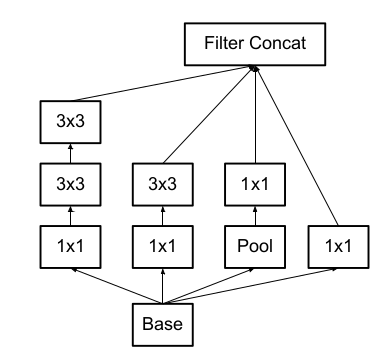
\includegraphics[width=3cm]{figs/inception_modules.png}}}
%\end{tabular}
%\end{center}
%\caption{Módulo inception onde cada convolução 5x5 foi substituída por duas convoluções 3x3.}
%\label{met:incept}
%\end{figure}

A \textit{InceptionV3} fatora convoluções maiores em menores, visto que uma convolução com kernel 5x5 com $n$ filtros sobre um grid com $m$ filtros é 25/9 = 2.78 vezes computacionalmente mais caro do que uma convolução 3x3 com o mesmo número de filtros. Além disso, a \textit{InceptionV3} também utiliza de fatoração espacial em convoluções assimétricas. Por exemplo, usar uma convolução 3x1 seguida por uma 1x3 é equivalente a ``deslizar'' uma rede com duas camadas com o mesmo campo receptivo como em uma convolução 3x3. Entretanto, a solução com duas camadas é 33\% mais barata para o mesmo número de filtros de saída - se o número de filtros de entrada e saída são iguais. Os bancos de filtros no módulo foram expandidos (mais largos em vez de mais profundos) para remover o gargalo representacional. Se o módulo fosse mais profundo, haveria muitas reduções de dimensões, e consequentemente perda de informação. 
%Entretanto, conforme notado em ~\cite{inception}, aplicar este tipo de fatoração não funciona bem em camadas iniciais mas funciona muito bem em \textit{grids} de tamanho médio ($m$ x $m$ feature maps, onde $m$ varia entre 12 e 20).

%\begin{figure}[htb]
%\begin{center}
%\begin{tabular}{c}
%\bmvaHangBox{\fbox{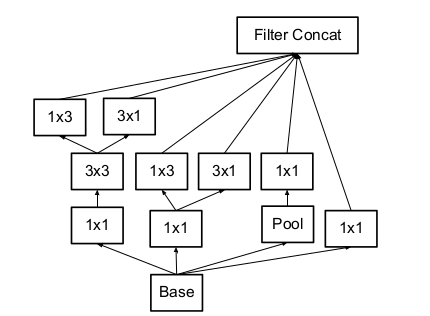
\includegraphics[width=3cm]{figs/inception_modules_factorized.png}}}
%\end{tabular}
%\end{center}
%\caption{Módulo inception após fatoração em convoluções menores. Os bancos de filtros no módulo foram expandidos (mais largos em vez de mais profundos) para remover o gargalo representacional. Se o módulo fosse mais profundo, haveria muitas reduções de dimensões, e consequentemente perda de informação.}
%\label{met:incept2}
%\end{figure}

%~\cite{going} introduziu a noção de classificadores auxiliares para melhorar a convergência de redes neurais muito profundas. A motivação original era de empurrar gradientes úteis para as camadas menores para fazê-las se tornarem úteis mais rápido e melhorar a convergência durante o treinamento combatendo o problema de desaparecimento de gradientes em redes neurais muito profundas. 
~\cite{inception} argumenta que classificadores auxiliares (introduzido por ~\cite{going}) agem como regularizadores. Esse argumento é suportado pelo fato que o classificador principal da rede se sai melhor (a \textit{InceptionV3} conseguiu um ganho absoluto de 0.4\% na acurácia top-1 com classificadores auxiliares no topo da última camada 17x17) se o ramo lateral é \textit{``batch-normalized''} ou se tem uma camada de dropout~\cite{dropout}.

Todas essas mudanças, com exceção de \textit{batch-normalization}, foram incorporadas já na \textit{Inception V2}. A \textit{InceptionV3} incorporou também: otimizador \textit{RMSProp}; convoluções fatoradas 7x7; e \textit{label smoothing} (um tipo de componente regularizador incorporado na \textit{loss formula} que previne a rede de se tornar muito confiante sobre uma classe e previne \textit{overfitting}).
%\begin{figure}[htb]
%\begin{center}
%\begin{tabular}{c}
%\bmvaHangBox{\fbox{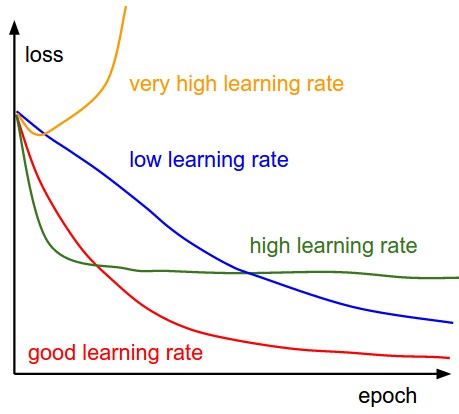
\includegraphics[width=3cm]{figs/learningrates.jpeg}}}
%\end{tabular}
%\end{center}
%\caption{Gráfico indicando curvas da loss/custo de acordo com a learning rate. Fonte: ~\cite{cs231n}}
%\label{fig:lrs}
%\end{figure}
%-------------------------------------------------------------------------
\subsection{Inception ResNetV2}
Conexões residuais foram introduzidas por ~\cite{deep}, onde foi apresentado evidências teóricas e práticas para as vantagens de se usar mistura aditiva de sinais para reconhecimento de imagens e detecção de objetos. Em ~\cite{szegedy2017inception} foi dada evidências empíricas de que combinar o treinamento com conexões residuais acelera o treinamento de redes \textit{Inception} significativamente, além de se sair melhor do que redes completamente \textit{Inception}, de mesmo custo computacional(\textit{InceptionV4}), por uma pequena margem. 

Para a versão residual das redes \textit{Inception} foi utilizado blocos \textit{Inception} mais baratos que o modelo original apresentado na subseção anterior \ref{met:inception}. Cada bloco \textit{Inception} é seguido por uma camada de expansão de filtro (convolução 1x1 sem ativação) que é usada para aumentar a dimensionalidade do banco de filtros antes da adição, para corresponder com a profundidade da entrada. Isso é necessário para compensar a redução na dimensionalidade induzida pelo bloco \textit{Inception}. Além disso, foi usado \textit{batch-normalization} apenas no topo das camadas tradicionais, mas não no topo dos somatórios. Isso foi feito para aumentar o número total de blocos \textit{Inception}. O diagrama da rede é mostrado na \textbf{figura} \ref{fig:diagramv2}.
\begin{figure}[htb]
\begin{center}
\begin{tabular}{c}
	\bmvaHangBox{\fbox{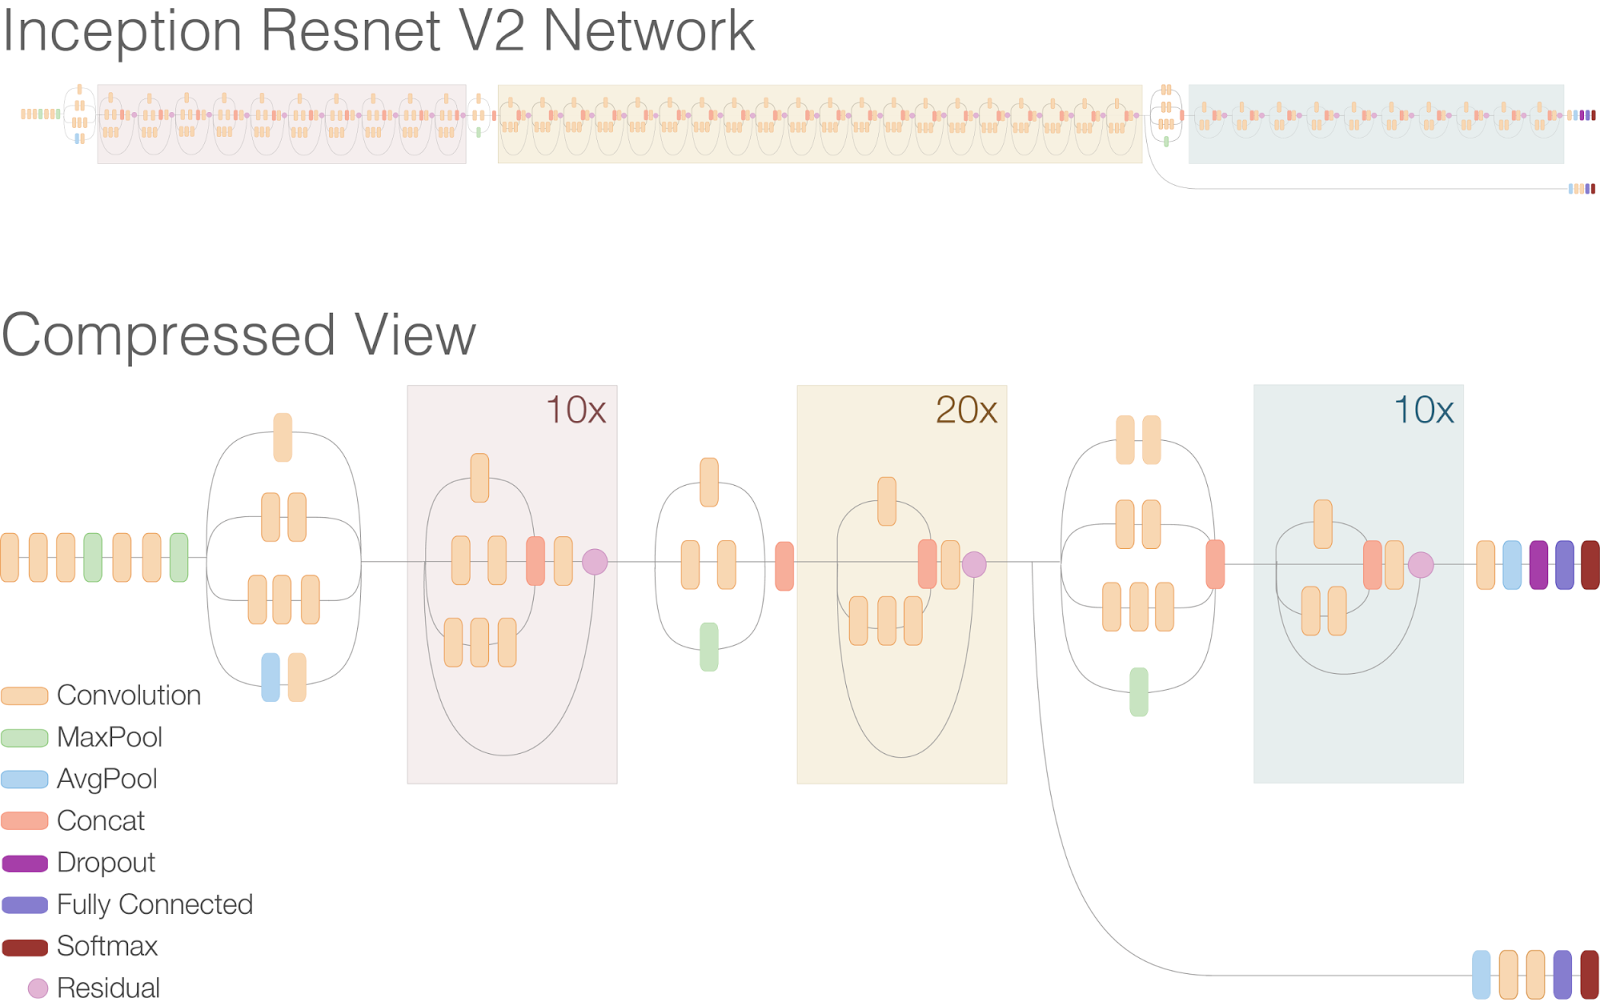
\includegraphics[width=5cm]{figs/inception_resnetv2_diagram.png}}}
\end{tabular}
\end{center}
\caption{Diagrama comprimido da Inception ResNetV2.}
\label{fig:diagramv2}
\end{figure}

Para as conexões residuais funcionarem, a entrada e saída após a convolução possui as mesmas dimensões. Logo, é usado 1x1 convoluções após a convolução original para corresponder ao tamanho das profundidades. A operação de pooling dentro dos principais módulos inception foram substituídos em favor das conexões residuais. Entretanto, essas operações continuaram nos blocos de redução. Ademais, os autores escalaram as ativações residuais por um valor entre 0.1 e 0.3, com o objetivo de aumentar a estabilidade.
%-------------------------------------------------------------------------
\subsection{Xception}
\label{res:Xception}
%-------------------------------------------------------------------------
A \textit{Xception}~\cite{xception} é uma nova arquitetura de rede neural convolucionária profunda inspirada na \textit{Inception}, onde os módulos \textit{Inception} foram substituídos por convoluções separáveis \textit{depthwise} modificadas. A \textit{Xception} conseguiu resultados melhores no dataset \textit{ImageNet}~\cite{imagenet_cvpr} e até mesmo em datasets maiores com mais classes para classificação. O mais interessante é que a \textit{Xception} tem o mesmo número de parâmetros da \textit{InceptionV3}, o que demonstra que houve um uso mais eficientes dos parâmetros em vez de aumento da capacidade do modelo.

Na \textit{Xception} houve uma modificação na camada \textit{Depthwise Separable Convolution}, conforme ilustra a figura \ref{fig:conv}. Nesta camada existe uma \textit{pointwise convolution} seguida por uma \textit{depthwise convolution} (ordem contrária no modelo \textit{InceptionV3}). \textit{Depthwise convolution} é a convolução espacial canal a canal. A convolução separável em profundidade(\textit{Depthwise convolution}) baseia-se em fatorizar a operação de convolução em duas camadas: uma convolução em profundidade que aplica um filtro para cada canal da entrada; e uma convolução por pontos (pointwise),
de tamanho 1x1, responsável por criar novas características por combinações lineares dos
canais de entrada e alteram a dimensão. Como resultado, são mais baratas computacionalmente sem perdas de
performance significativas em relação às convoluções completas, conforme dito anteriormente na seção \ref{met:inception}. 

\begin{figure}[htb]
\begin{center}
\begin{tabular}{c}
	\bmvaHangBox{\fbox{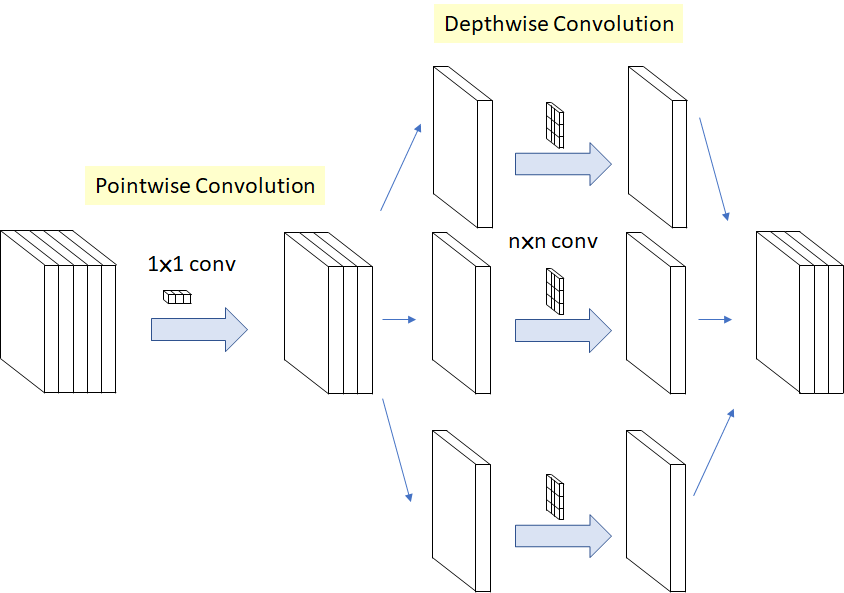
\includegraphics[width=3cm]{figs/conv.png}}}
\end{tabular}
\end{center}
\caption{A convolução separável em profundidade modificada usada como um módulo \textit{Inception} na arquitetura \textit{Xception}. Também chamada de ``versão extrema'' do módulo \textit{Inception}.}
\label{fig:conv}
\end{figure}
Essa modificação é motivada pelo módulo inception na \textit{InceptionV3} onde a convolução 1x1 é feita primeira antes de qualquer $n$x$n$ convoluções espaciais. Além disso, no módulo \textit{Inception} original existe não linearidade após a primeira operação. No \textit{Xception}, a convolução separável em profundidade modificada, não existe a não linearidade da função de ativação \textit{ReLU}. Os resultados reportados pelos autores em ~\cite{xception} mostram que a ausência da não-linearidade leva a convergência mais rápida e performance final melhorada. Isso é um resultado interessante, visto que os autores da \textit{InceptionV3} reportaram o oposto para módulos \textit{Inception} em ~\cite{inception}.

Quanto a configuração de regularização, a \textit{InceptionV3} usa uma taxa \textit{weight decay} (regularização L2) 4 vezes maior do que a usada na \textit{Xception}. O Dropout utilizado por ambas as arquiteturas foi de 50\% para o dataset \textit{ImageNet}. Além disso, a arquitetura \textit{InceptionV3} usa um mecanismo de torre auxiliar de perda/custo que serve como um mecanismo adicional de regularização, fazendo a \textit{back-propagation} da \textit{classification loss} mais cedo na rede. Esse mecanismo não foi utilizado na \textit{Xception}. Todos as camadas de convolução e de convolução separável são seguidas por \textit{batch normalization} na \textit{Xception}.
\section{Experimentos e Análise dos Resultados}
Nesta seção são apresentados e analisados alguns resultados e hiper-parâmetros para todas as arquiteturas. O tamanho do conjunto de validação utilizada para todos os modelos foi de 20\% do conjunto de treino fornecido (1500 imagens). Foi utilizado a função \textit{ImageDataGenerator}~\cite{keras} para o uso de \textit{data augmentation} com o objetivo de melhorar os resultados, considerando que o tamanho do \textit{dataset} é pequeno. 20\% das imagens de treino foram utilizadas como validação com o objetivo de obter melhores resultados. O otimizador escolhido para todos os experimentos foi o ~\cite{sgd}.
%-------------------------------------------------------------------------
\subsection{InceptionV3}
Avaliou-se o modelo em 3 cenários diferentes, conforme mostra a \textbf{tabela} \ref{tab:results1}. Na versão 1.0 é possível observar pelos gráficos da \textbf{figura} \ref{fig:results1} que o \textit{decay} utilizado de atualizar a learning rate  da \textit{learning rate} escolhida foi muito alto. Nota-se que a \textit{loss} não convergiu, ou seja, não chegou ao mínimo. É sabido que taxas de aprendizagem baixas precisam de mais épocas para que a função custo chegue ao mínimo e acurácia atinja o máximo. 
 
A curva de loss/accuracy para a versão 2.0 prova que a decisão de retirar o \textit{decay} da \textit{learning rate} foi boa. Entretanto, é possível notar uma oscilação na \textit{loss}. Isto provavelmente se deve ao aumento em 20\% no dropout~\cite{dropout} utilizado. O \textit{dropout} previne unidades de se co-adaptarem muito dropando-as junto com suas conexões, o que previne overfitting pois essas co-adaptações das unidades para diminuir a \textit{loss} são complexas e podem não generalizar bem para dados não vistos. Contudo, o \textit{dropout} pode aumentar o erro no início do treinamento apesar do erro/\textit{loss} final após convergência da função de custo normalmente ser menor. 
%Aleḿ disso, o dropout funciona como um regularizador e a \textit{InceptionV3} já possui métodos de %regularização. Logo, a taxa de dropout tem que ser estudada com cuidado para que não haja regularização %excessiva.

É possível notar pelo gráfico da \textbf{figura} \ref{fig:results1} que a versão 3.0 foi a que apresentou mais sinais de \textit{overfitting}. Há uma diferença considerável entre a \textit{loss} na validação e no treino. Também é possível notar que a diferença entre a acurácia na validação e no treino é a maior de todos os cenários testados. Porém há dois fatores importantes a serem considerados aqui. Primeiro, o \textit{batch size} utilizado é maior. Tamanhos de \textit{batches} baixos podem não representar bem o conjunto de dados como um todo e podem levar o modelo a perder capacidade de generalização (considerando também o fato de que com um \textit{batch size} menor há mais iterações). Todavia, tamanhos de \textit{batches} altos podem diminuir a capacidade de generalização~\cite{batch}, visto que eles não fornecerão o verdadeiro gradiente e tendem a levar a mínimos que são muito sensíveis a perturbação dos parâmetros (\textit{sharp minima}). Ademais, como a quantidade de imagens para treino utilizada é de 1200 imagens desconsiderando as imagens geradas usando \textit{data augmentation}, um \textit{batch size} de 128 já representa cerca de 10\% do total de imagens, o que pode afetar a capacidade de generalização e causar um pouco de sobreajuste\footnote{vale notar que um \textit{batch size} maior há menos atualizações nos pesos (redução da variância nas atualizações do gradiente) e pode levar a uma melhor qualidade do modelo também, já que não alterará muito os pesos pré-treinados originais} no conjunto de treino. Segundo, foi usado uma política diferente para atualização da \textit{learning rate}: a \textit{learning rate} cíclica~\cite{cyclical}. Como tamanhos de batches altos podem levar a mínimos da função de custo que são sensíveis a pertubação de parâmetros, essa política diferente de learning rate pode ser a causa da diferença observada entre o erro do treino e da validação no modelo 3.0.

Para o modelo 1.0 foi utilizado uma taxa de atualização de 0.001/50 para a \textit{learning rate}, que é atualizada em todas as épocas. Para o modelo 2.0 foi utilizado um \textit{callback} de reduzir pela metade a \textit{learning rate} caso a \textit{loss} não diminua em 5 épocas. Além disso, o treinamento da rede foi interrompido na época 45 pois não houve melhora na acurácia em 20 épocas, ou seja, a acurácia atingida na época 45 não foi maior do que a maior acurácia atingida no intervalo de épocas 20 até 45. 
\begin{table}[htb]
\caption{Resultados da InceptionV3 em cada cenário. O modelo 1.0 obteve 0.87 de \textit{F1 Score}, o modelo 2.0, 0.92 e o 3.0, 0.90.} 
\label{tab:results1}
\begin{tabular}{|l|l|l|l|l|l|}
\hline
                         & \textbf{Dropout} & \textbf{Learning Rate}                                   & \textbf{Batch Size} & \textbf{Epochs} & \textbf{Acurácia} \\ \hline
\textbf{InceptionV3-1.0} & 50\%             & \begin{tabular}[c]{@{}l@{}}0.001\\ Decay\end{tabular}    & 32                  & 50              & 86.97\%           \\ \hline
\textbf{InceptionV3-2.0} & 70\%             & \begin{tabular}[c]{@{}l@{}}0.001\\ ReduceLR\end{tabular} & 32                  & 45              & 92.43\%           \\ \hline
\textbf{InceptionV3-3.0} & 70\%             & \begin{tabular}[c]{@{}l@{}}0.001\\ CyclicLR(triang)\end{tabular} & 64                  & 40              & 89.65\%           \\ \hline
\end{tabular}
\end{table}

\begin{figure}[htb]
\centering
\begin{tabular}{ccc}
  \bmvaHangBox{\fbox{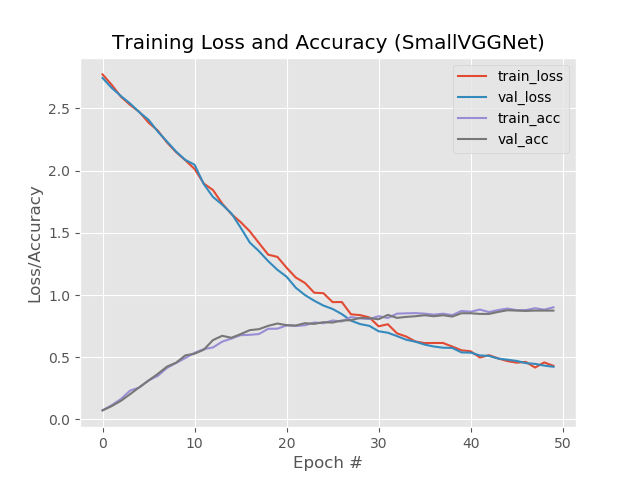
\includegraphics[width=35mm]{figs/inception_V3_plot-10.png}}} &  
  \bmvaHangBox{\fbox{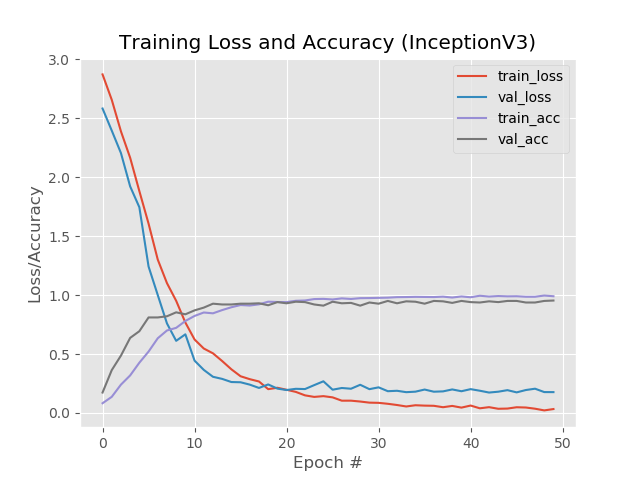
\includegraphics[width=35mm]{figs/inception_V3_plot-20.png}}} &
  \bmvaHangBox{\fbox{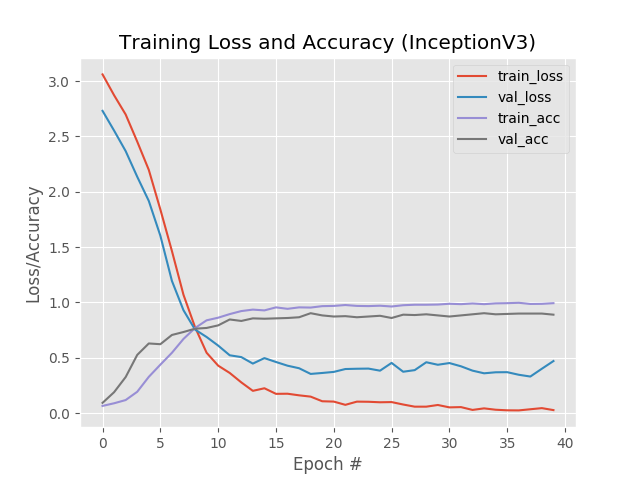
\includegraphics[width=35mm]{figs/inception_V3_plot-30.png}}} \\
(a) Modelo 1.0 & (b) Modelo 2.0 & (c) Modelo 3.0\\[6pt]
\end{tabular}
\caption{Resultados da InceptionV3.}
\label{fig:results1}
\end{figure}

\subsection{Inception ResNetV2}
%-------------------------------------------------------------------------
A rede \textit{Inception ResNetV2} foi testada também em 3 cenários diferentes, conforme mostra a \textbf{tabela} \ref{tab:results2}. Para todos os modelos foi utilizado taxa de aprendizagem cíclica e um \textit{early stopping para} a \textit{loss} de 15 ou 20 épocas. Os modelos 2.0 e 3.0 foram treinados com o número máximo de 40 épocas e houve um \textit{early stopping} na época 35 e 36, respectivamente. A decisão de diminuir o número de épocas veio após observação de que a \textit{loss} estava convergindo para o mínimo - e a acurácia para o máximo - mais rápido do que o esperado. 

Com os experimentos nessa arquitetura fortaleceu-se o argumento, apresentado na subseção anterior e por ~\cite{batch}, de que \textit{batches} grandes para treinamento podem diminuir a qualidade do modelo, visto que o \textit{batch size} é a única diferença de parâmetros entre as redes 1.0 e 2.0. A rede 1.0~\ref{fig:results2} apresentou menos sinais de \textit{overfitting}, o que já era esperado devido ao uso de maior taxa de \textit{dropout}. Contudo, há uma maior ``instabilidade'' nas curvas que pode ser explicado pelo uso do modo padrão \textit{``triangular''}~\cite{clr} da política de \textit{learning rate} cíclica. Este modo altera a \textit{learning rate} de forma mais brusca (que provavelmente são os picos na \textit{loss} da validação e consequentemente na acurácia dela), enquanto o modo usado na rede 3.0 \textit{``exp\_range''} altera a learning rate de forma mais suave.

\begin{table}[htb]
\caption{Resultados da InceptionResNetV2 em cada cenário. Todos os modelos obtiveram 0.93 de \textit{F1 Score}, com exceção do 2.0 que obteve 0.92.}
\label{tab:results2}
\begin{tabular}{|l|l|l|l|l|l|}
\hline
                               & \textbf{Dropout} & \textbf{Learning Rate}                                   & \textbf{Batch Size} & \textbf{Epochs} & \textbf{Acurácia} \\ \hline
\textbf{InceResNetV2-1.0} & 50\%             & \begin{tabular}[c]{@{}l@{}}0.001\\ CyclicLR(triang)\end{tabular} & 64                  & 50              & 93.07\%           \\ \hline
\textbf{InceResNetV2-2.0} & 50\%             & \begin{tabular}[c]{@{}l@{}}0.001\\ CyclicLR(exp)\end{tabular} & 128                 & 35              & 92.36\%           \\ \hline
\textbf{InceResNetV2-3.0} & 40\%             & \begin{tabular}[c]{@{}l@{}}0.001\\ CyclicLR(exp)\end{tabular} & 64                  & 40              & 93.43\%               \\ \hline
\end{tabular}
\end{table}
\label{sec:res}

\begin{figure}[htb]
\centering
\begin{tabular}{cc}
  \bmvaHangBox{\fbox{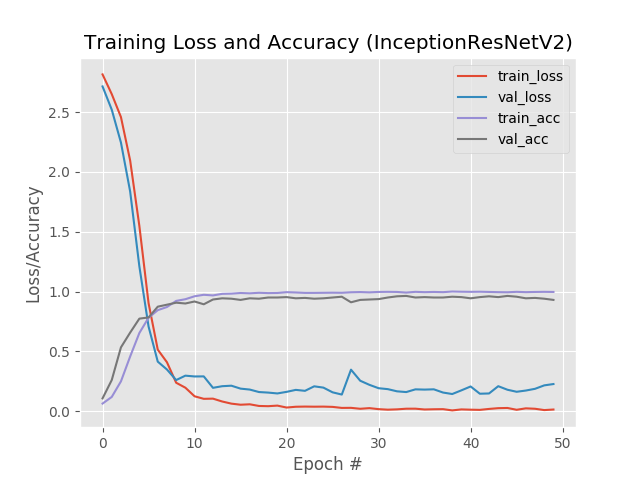
\includegraphics[width=30mm]{figs/inception_resnetv2_plot-10.png}}} &  
  \bmvaHangBox{\fbox{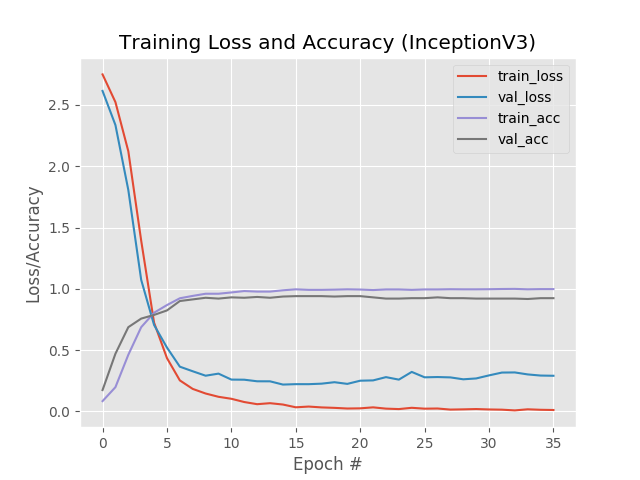
\includegraphics[width=30mm]{figs/inception_resnetv2_plot-30.png}}} \\
(a) Modelo 1.0 & (b) Modelo 3.0 \\[6pt]
\end{tabular}
\caption{Resultados da Inception ResNetV2.}
\label{fig:results2}
\end{figure}

\subsection{Xception}
%-------------------------------------------------------------------------
A rede \textit{Xception} foi testada em 3 cenários. O número de épocas máximo foi reduzido, devido a observações de rápida convergência nos modelos anteriores. Nota-se pela \textbf{figura} \ref{fig:best} que houve pouca diferença entre a acurácia e loss no treino e a validação. Possivelmente mais épocas poderiam resultar em uma acurácia superior à 93.43\% obtida pelo modelo da seção anterior, considerando a estabilidade das curvas de aprendizagem dos modelos. 

\begin{table}[htb]
\caption{Resultados da Xception em cada cenário. Todos os modelos \textit{Xception} testados obtiveram 0.93 de \textit{F1 Score}.}
\begin{tabular}{|l|l|l|l|l|l|}
\hline
                      & \textbf{Dropout} & \textbf{Learning Rate}                                           & \textbf{Batch Size} & \textbf{Epochs} & \textbf{Acurácia} \\ \hline
\textbf{Xception-1.0} & 50\%             & \begin{tabular}[c]{@{}l@{}}0.001\\ CyclicLR(exp)\end{tabular}    & 64                  & 50              & 93.07\%           \\ \hline
\textbf{Xception-2.0} & 70\%             & \begin{tabular}[c]{@{}l@{}}0.001\\ CyclicLR(exp)\end{tabular}    & 48                  & 25              & 92.66\%           \\ \hline
\textbf{Xception-3.0} & 60\%             & \begin{tabular}[c]{@{}l@{}}0.001\\ CyclicLR(trian2)\end{tabular} & 64                  & 25              & 93.23\%           \\ \hline
\end{tabular}
\end{table}

\begin{figure}[htb]
\begin{center}
\begin{tabular}{cc}
	\bmvaHangBox{\fbox{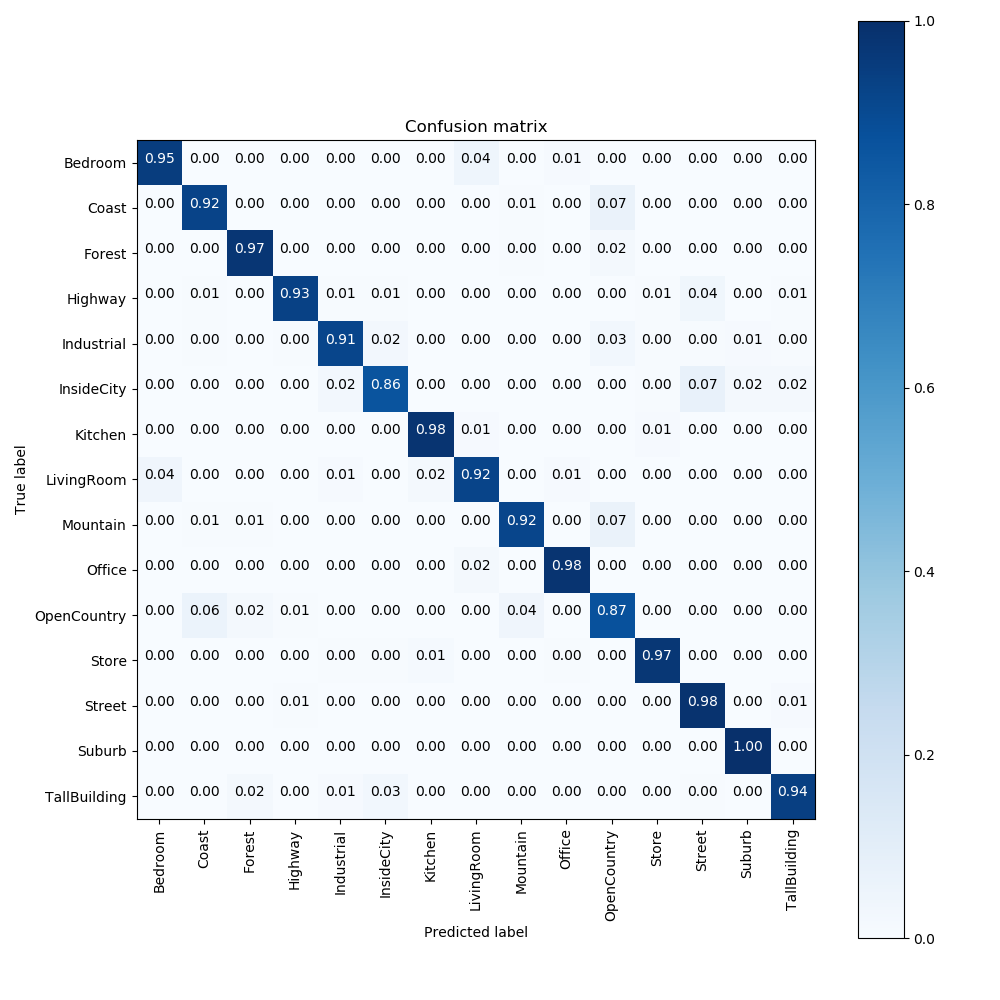
\includegraphics[width=60mm]{figs/best_confusion_matrix.png}}} &
	\bmvaHangBox{\fbox{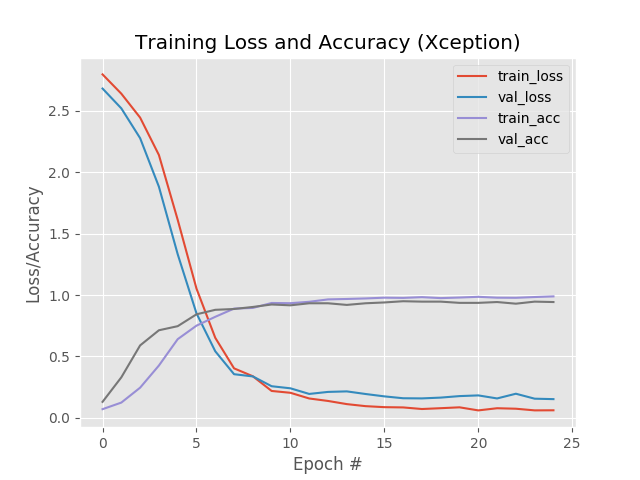
\includegraphics[width=42mm]{figs/Xception30_plot.png}}} \\ 
\end{tabular}
\end{center}
\caption{Matriz de confusão do modelo que obteve o melhor resultado neste projeto e curva de aprendizagem da Xception 3.0.}
\label{fig:best}
\end{figure}

%\begin{figure}[htb]
%\begin{center}
%\begin{tabular}{c}
%	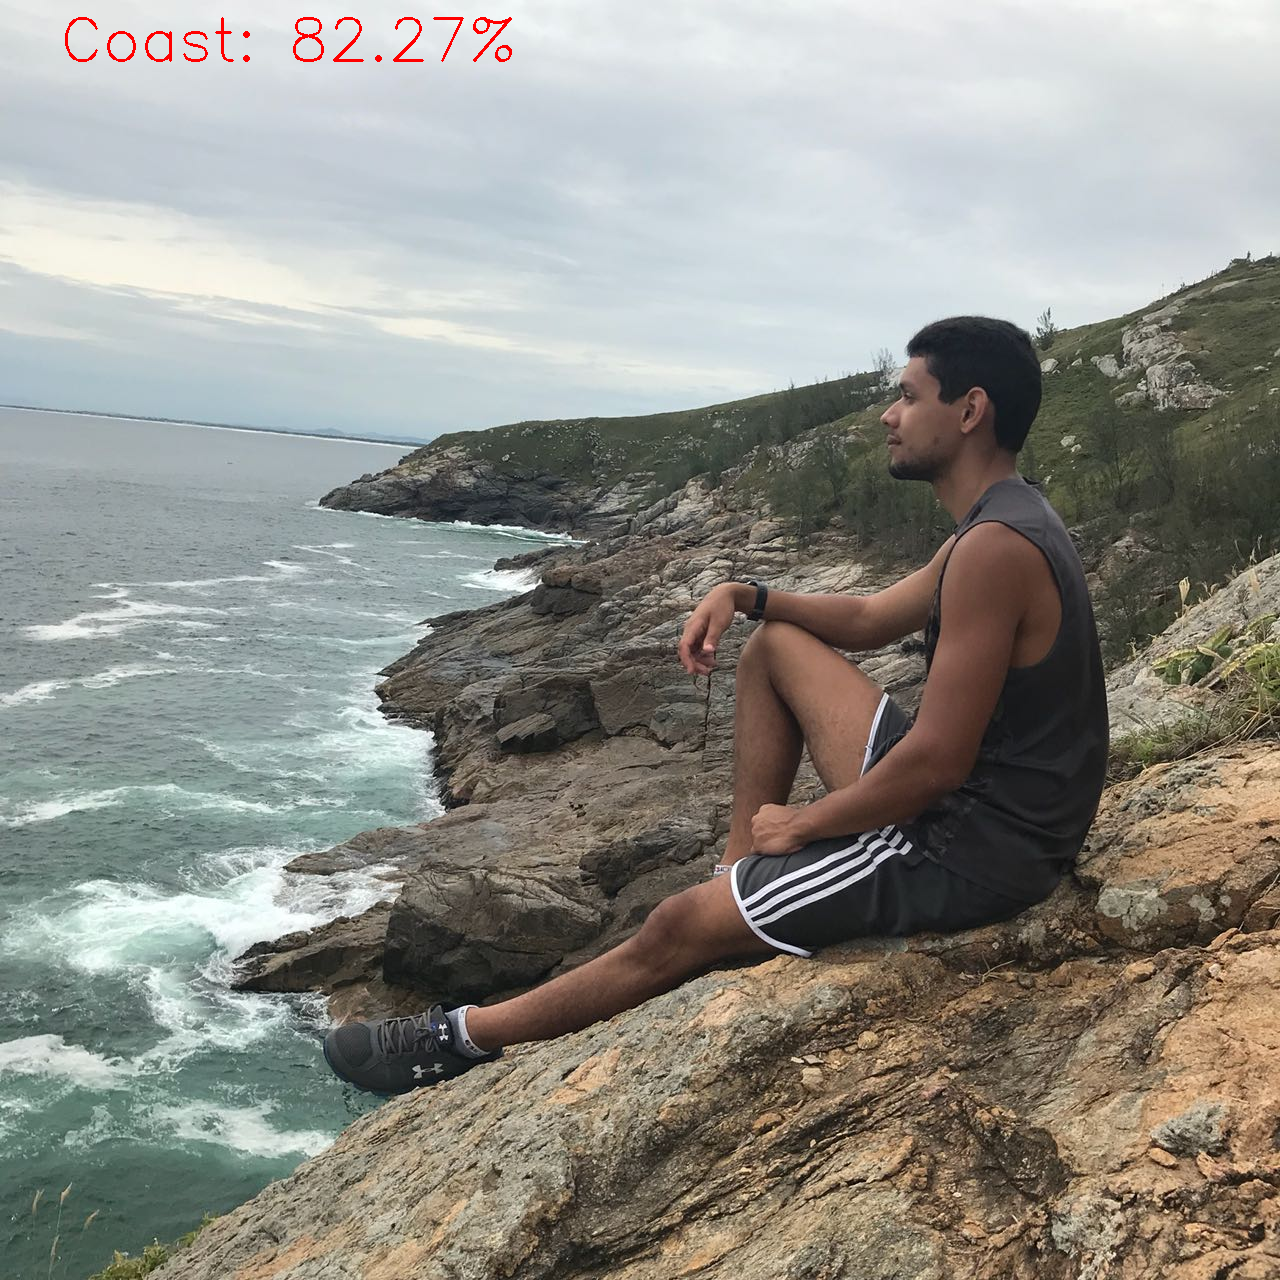
\includegraphics[width=25mm]{figs/Image.png} 
%\end{tabular}
%\end{center}
%\caption{Testando o melhor modelo em uma imagem fora do dataset.}
%\end{figure}

%-------------------------------------------------------------------------
\section{Conclusão}
\label{sec:conc}
Como estudo futuro pode-se investigar o uso de outros otimizadores, considerando que o otimizador que forneceu os melhores resultados para os autores dos três modelos foi o \textit{RMSprop}. A \textit{Inception ResNetV2} se sobressaiu sobre os outros modelos, entretanto se fosse realizado mais testes acredita-se que a \textit{Xception} conseguiria se sobressair sobre as suas similares, mesmo com um custo computacional menor ou igual. Com este trabalho foi possível notar que o hiper-parâmetro de maior importância e maior impacto para os modelos foi a taxa de aprendizagem. Não só o valor inicial da taxa, mas também a política de atualização dela.
\clearpage
\bibliography{refs}
\end{document}
%\begin{figure}[htb]
%\begin{center}
%\begin{tabular}{c}
%\bmvaHangBox{\fbox{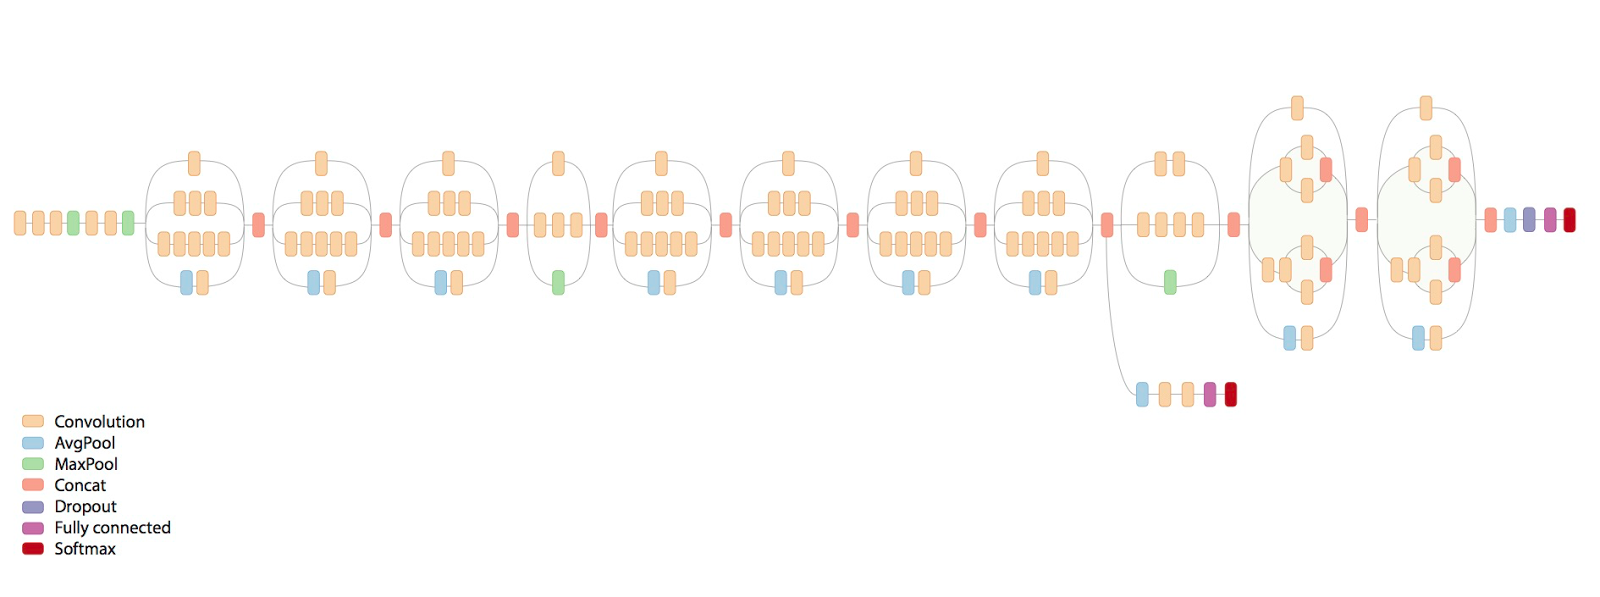
\includegraphics[width=8cm]{figs/inceptionv3_diagram.png}}}
%\end{tabular}
%\end{center}
%\caption{Diagrama comprimido da Inception V3.}
%\label{fig:diagramv3}
%\end{figure}

%\begin{figure}[htb]
%\begin{center}
%\begin{tabular}{c}
%\bmvaHangBox{\fbox{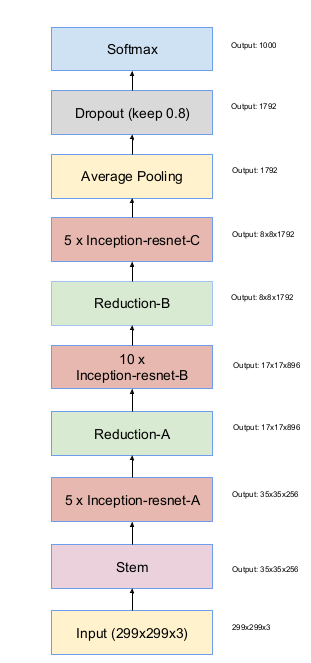
\includegraphics[width=3cm]{figs/schema_inceptionresnet.png}}}
%\end{tabular}
%\end{center}
%\caption{Esquema das redes Inception ResNetV1 e Inception ResNetV2. Fonte: ~\cite{szegedy2017inception}}
%\label{fig:schemav2}
%\end{figure}